% The loop between a group and the task force (Assignment 8 sheet, intro), built to SVG by make.sh.
\documentclass[border=3pt]{standalone}
\usepackage{tikz}
\usepackage{fontspec}
\setsansfont{GilliusADFNo2}[Path=../../assets/, Extension=.otf, UprightFont=*-Regular, BoldFont=*-Bold]
\renewcommand{\familydefault}{\sfdefault}
\usetikzlibrary{arrows.meta, positioning, fit, backgrounds}
\definecolor{HSGgreen}{HTML}{00802F}
\definecolor{HSGgreenLight}{HTML}{E7EDE8}
\definecolor{HSGteal}{HTML}{73A5AF}
\definecolor{HSGtealLight}{HTML}{DCE9EC}
\definecolor{ink}{HTML}{1A1A1A}
\definecolor{frame}{HTML}{595959}
\begin{document}
% Scaled up so that the slide, which never enlarges a picture, can show it at full width.
\scalebox{2.5}{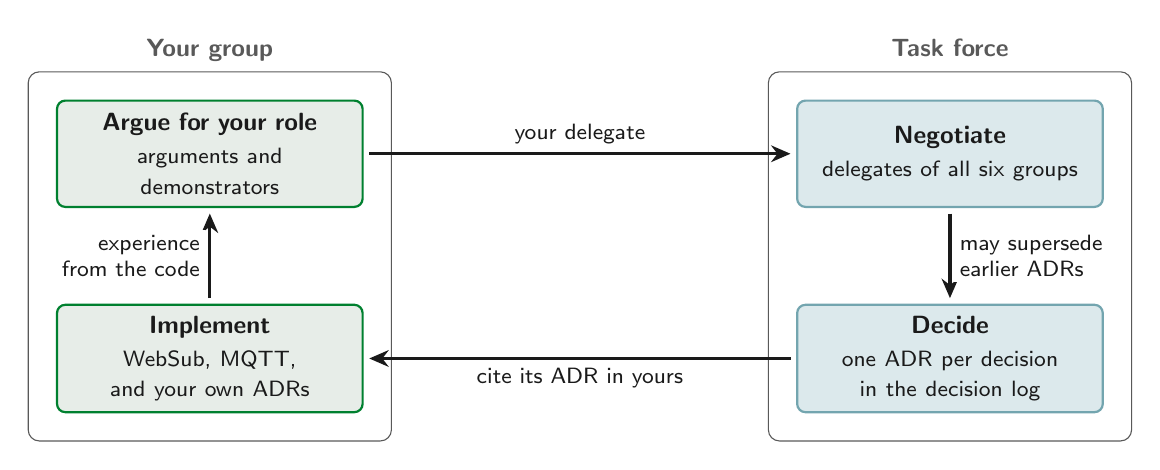
\begin{tikzpicture}[
    x=1cm, y=1cm, font=\small, text=ink,
    stepbox/.style={rounded corners=3pt, draw, thick, text width=3.6cm, minimum height=1.35cm,
                 align=center, inner sep=4pt},
    grp/.style={stepbox, draw=HSGgreen, fill=HSGgreenLight},
    tf/.style={stepbox, draw=HSGteal, fill=HSGtealLight},
    >={Stealth[length=7pt, width=6pt]},
    flow/.style={->, very thick, draw=ink, shorten <=2pt, shorten >=2pt},
    lab/.style={font=\footnotesize, fill=white, inner sep=2pt}]

  % Your group (left) and the task force (right); the loop runs clockwise.
  \node[grp] (argue) at (0, 0)    {\textbf{Argue for your role}\\[1pt]{\footnotesize arguments and demonstrators}};
  \node[tf]  (nego)  at (9.4, 0)  {\textbf{Negotiate}\\[1pt]{\footnotesize delegates of all six groups}};
  \node[tf]  (dec)   at (9.4, -2.6) {\textbf{Decide}\\[1pt]{\footnotesize one ADR per decision in the decision log}};
  \node[grp] (impl)  at (0, -2.6) {\textbf{Implement}\\[1pt]{\footnotesize WebSub, MQTT, and your own ADRs}};

  \draw[flow] (argue) -- node[lab, above=1pt] {your delegate} (nego);
  \draw[flow] (nego)  -- node[lab, right=1pt, align=left] {may supersede\\earlier ADRs} (dec);
  \draw[flow] (dec)   -- node[lab, below=1pt] {cite its ADR in yours} (impl);
  \draw[flow] (impl)  -- node[lab, left=1pt, align=right] {experience\\from the code} (argue);

  \begin{scope}[on background layer]
    \node[draw=frame, rounded corners=4pt, inner sep=10pt, fit=(argue)(impl), label={[font=\small\bfseries, text=frame, text height=1.6ex, text depth=.4ex]above:Your group}] {};
    \node[draw=frame, rounded corners=4pt, inner sep=10pt, fit=(nego)(dec), label={[font=\small\bfseries, text=frame, text height=1.6ex, text depth=.4ex]above:Task force}] {};
  \end{scope}
\end{tikzpicture}}
\end{document}
